\chapter{Methodology}
\label{methodology}

%\cgn{Is it more logical to move this Methodology after Implementation chapter and before Validation one? Naturally, after discussing the related work and discussing their limitation, one would expect to see the proposed solution (with Design and Implementation).}
%\cfw{This chapter is basically split in two parts: Everything until 4.4 covers content that is needed for design and implementation. 4.5 to 4.7 then cover our validation methods. I thus see this chapter as more of a chronological order on how the solution was created and evaluated, before actually performing these actions. The role of the chapter is thus more directed at "what did we do after our research" for me rather than what is immediatly up next in the thesis. Maybe we can discuss this tomorrow in our meeting. It would sure be possible to move 4.5 to 4.7 to the beginning of chapter 7 without many issues.}
To be able to accurately design, implement and validate our solution we will need to specify our methodology first. To achieve our goal we will use requirement validation as an overall strategy. Initially we defined our requirements as stated in Section \ref{related_work_requirements}.

In this chapter we will thus define a network model, our protection goals and attackers. Our validation methodology is stated later in Section \ref{validation_methodology}.


\section{Network model}
In the context of our networks, we will establish two different kinds of networks.

\begin{figure}[ht]
    \centering
    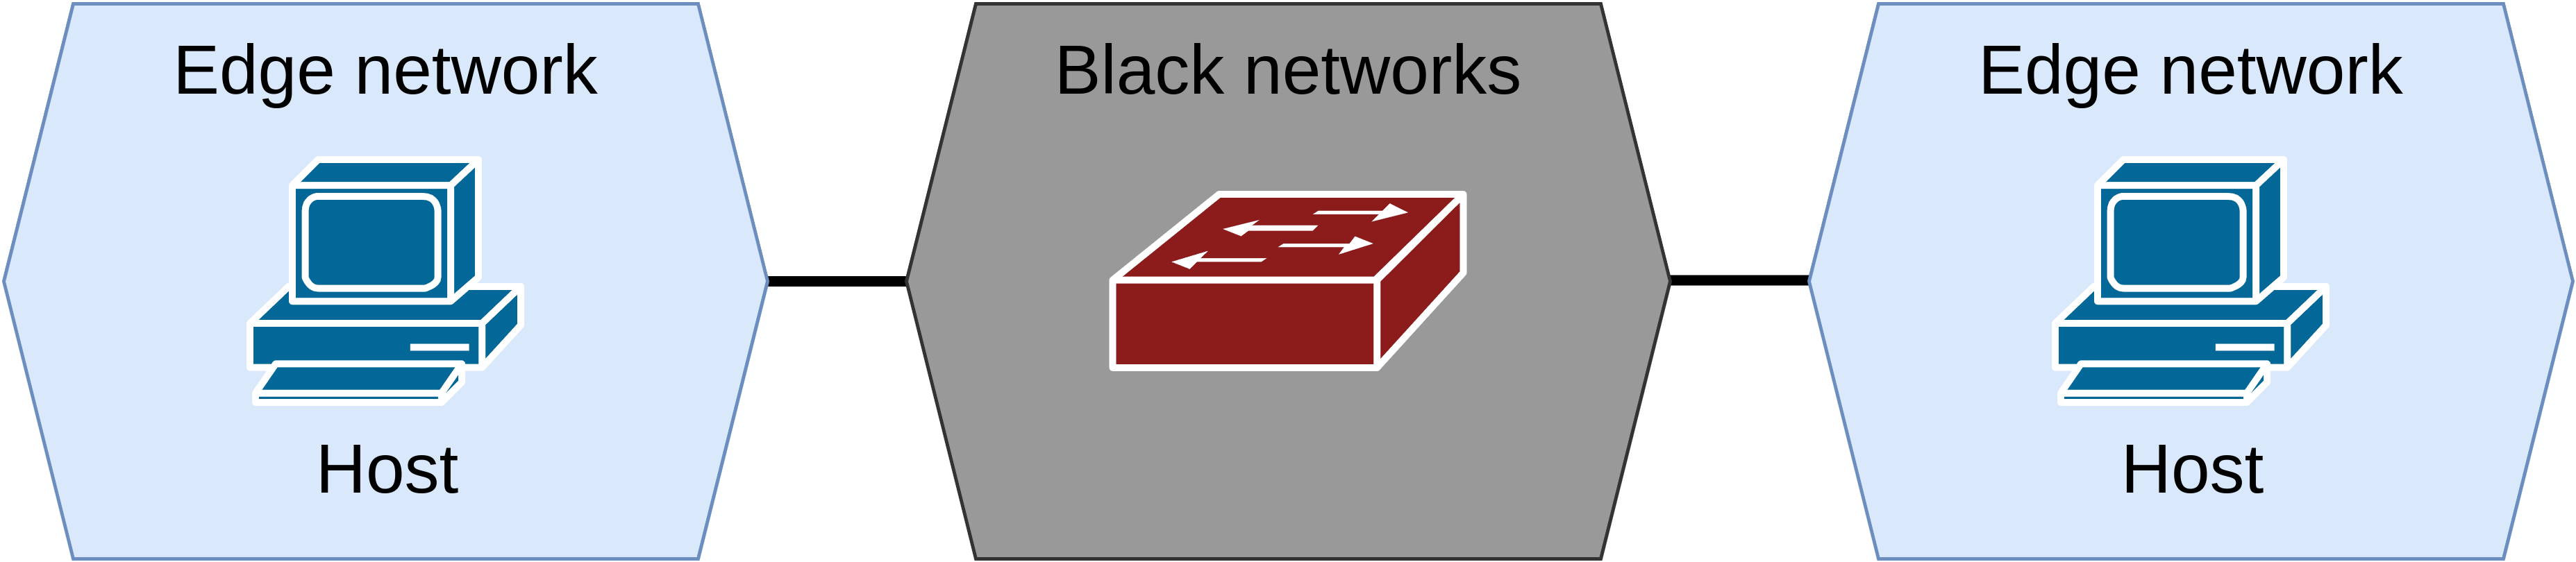
\includegraphics[width=8cm]{images/chapter_4/network_model.png}
    \caption[Network model]{Our network model showing the separation of trusted \gls{edgenetwork}s and semi-trusted \gls{blacknetwork}s. While \gls{edgenetwork}s are the source and target of our network slice traffic, \gls{blacknetwork}s act as transit networks. There can be multiple \gls{blacknetwork}s between our \gls{edgenetwork}s, but for simplicity reasons only one of them is indicated in the figure.}
    \label{fig:network_model}
\end{figure}

\paragraph{Edge networks}
are the origin and target of one specific network slice. Each \gls{edgenetwork} is partially trusted by us, because we or another trusted party operate the core infrastructure. We only expect threats from adversaries outside of our switches or slicing architecture following a \gls{zerotrust} approach, for example as a host established within our \gls{edgenetwork}.

\paragraph{Black networks}
lie between the \gls{edgenetwork}s and are operating under a service level agreement (\acrshort{sla}). There may be any number of \gls{blacknetwork}s between two edges, including none. A \gls{blacknetwork} acts as a transit network to us and is semi-trusted because the infrastructure is not operated by us. We do trust that the \gls{blacknetwork} will act according to protocol, but it might be interested in breaking confidentiality or even integrity. As with our \gls{edgenetwork}s, we expect attackers to be established outside of the switching and slicing architecture following a \gls{zerotrust} approach, apart from potential eavesdropping or integrity violation attempts by the transport infrastructure of the \gls{blacknetwork}.

Please note that one specific network may play different roles for different network slices. One slice may pass through a \gls{blacknetwork} that is also the origin (and thus \gls{edgenetwork}) of another slice.

Our network model can also be seen in Figure \ref{fig:network_model}.


\section{Protection Goals}
\label{protection_goals}
The next question we posed was what we actually desire to protect from our attackers. In general we strive to protect the communication from one host to another and provide certain guarantees to the hosts. These guarantees include \gls{bandwidth}, \gls{latency}, \gls{jitter}, \gls{lossrate} and of course availability. Furthermore we want to protect traffic from modification or information disclosure in networks between our \gls{edgenetwork}s. We do not require this protection on our \gls{edgenetwork}s, since we trust our self-managed infrastructure to a certain degree. Our protection goals are thus:
\begin{description}[style=multiline, labelwidth=0.7cm]
    \item[\namedlabel{P1}{P1}] \textbf{Confidentiality} Traffic needs to be protected from disclosure outside of the \gls{edgenetwork}s.
    \item[\namedlabel{P2}{P2}] \textbf{Integrity} Traffic needs to be protected from modification by attackers outside of our path on the \gls{edgenetwork}s and from attackers on the \gls{blacknetwork}.
    \item[\namedlabel{P3}{P3}] \textbf{Availability} Slices need to be available for communication and deliver packets to the recipient at all times during their lifespan.
    \item[\namedlabel{P4}{P4}] \textbf{Resilience} Slices need to provide their guaranteed network resources with their specified \gls{bandwidth}, \gls{latency}, \gls{jitter} and \gls{lossrate}, even when the network is under attack.
\end{description}


\section{Threats and Attackers}
\label{adversaries}
Now that we specified our protection goals, the attackers should be designed.

As previously mentioned, Ruxandra Olimid et. al \cite{SE2} classified threats to network slicing as either life-cycle threats, inter-slice threats or intra-slice threats. We will present our attackers for these threats below.

\paragraph{Inter-slice threats} For inter-slice threats we will create an attacker utilizing a lot of resources within another slice to overload the network and potentially create artifacts in our slice that should be prevented. We do not consider side-channel attacks on our slicing implementation to test the isolation between slices as it heavily depends on the used components while we will try to support a variety of components (e.g. the implementation of queues in the linux kernel vs a hardware switch).

\paragraph{Life-cycle threats} For life-cycle threats we will introduce two attackers, one spamming our application plane with arbitrary requests and one spamming our slice coordinators with valid requests. We hope to achieve denial of service for new slice registrations with the first attacker and an overload of network resources by the second attacker.

\paragraph{Intra-slice threats} As the last two attackers we will consider attackers attempting to eavesdrop or violate integrity within one of the \gls{blacknetwork}s between our two \gls{edgenetwork}s. The eavesdropping attacker will only observe traffic attempting to break confidentiality. The integrity attacker will however try to replay and craft new messages (including sending modified packets additionally). Dropping and modifying packets should not be supported by the attacker, as we can not compensate for the subsequently lost packets while only using a single path without resending packets, potentially violating resource guarantees. Eavesdroppers and integrity attackers are not expected on our \gls{edgenetwork}s, as we trust our local environment infrastructure (but not all tenants).

\paragraph{Exclusions} As it has already been the case with the attacker on integrity, we do not consider active in-path attackers (apart from the integrity attacker), as they could disrupt communication at any time. If resilience against these kinds of attacks is needed, the solution would need to be extended to include multiple paths. This is however out of scope for this thesis. Apart from all components and links used by the network slice, in-path attackers contain our entire application plane, as any component of the application plane that participates in a slice could instruct other components to disrupt the connection or disrupt the connection themselves. To compensate this, routing via multiple alternative paths would be required, introducing redundancy to the network.

We also do not include attackers on confidentiality and integrity on the application plane here, as this could be easily solved by using transport layer security (TLS) enabled protocols for communication in the future, which is however also currently out of scope for this thesis. The same applies to a proper authentication scheme on the application plane.

There are also no attackers on our control plane, because all control plane components are in-path (as stated above) and are not directly reachable by tenant devices of our networks that we distrust.

\paragraph{} Our attacker definitions are thus as follows:
\begin{description}[style=multiline, labelwidth=0.7cm]
    \item[\namedlabel{A1}{A1}] \textbf{Slice availability and resilience} Overloads the network by sending a lot of traffic through another slice that has shared components and network links with our slice that should be protected. Attacks protection goals \ref{P3} (availability) and \ref{P4} (resilience).
    \item[\namedlabel{A2}{A2}] \textbf{Application plane availability and resilience (1)} Spams invalid slice requests on the exposed application plane components attempting to disrupt the creation of new slices. Attacks protection goals \ref{P3} (availability) and \ref{P4} (resilience).
    \item[\namedlabel{A3}{A3}] \textbf{Application plane availability and resilience (2)} Spams valid authenticated slice requests on the exposed application plane components attempting to overload the network by capacity or frequent slice creation and removal. Attacks protection goals \ref{P3} (availability) and \ref{P4} (resilience).
    \item[\namedlabel{A4}{A4}] \textbf{Slice confidentiality} Attempts to eavesdrop within one of the \gls{blacknetwork}s. Attacks protection goal \ref{P1} (confidentiality).
    \item[\namedlabel{A5}{A5}] \textbf{Slice integrity} Attempts to modify contents of a slice within one of the \gls{blacknetwork}s by replaying or sending additional packets. Will not modify or drop packets, but may send modified packets as additional packets. Attacks protection goal \ref{P2} (integrity).
\end{description}

Our attackers can also be seen in Figure \ref{fig:attacker_model}.

%\begin{landscape}
    \begin{figure}[h]
        \centering
        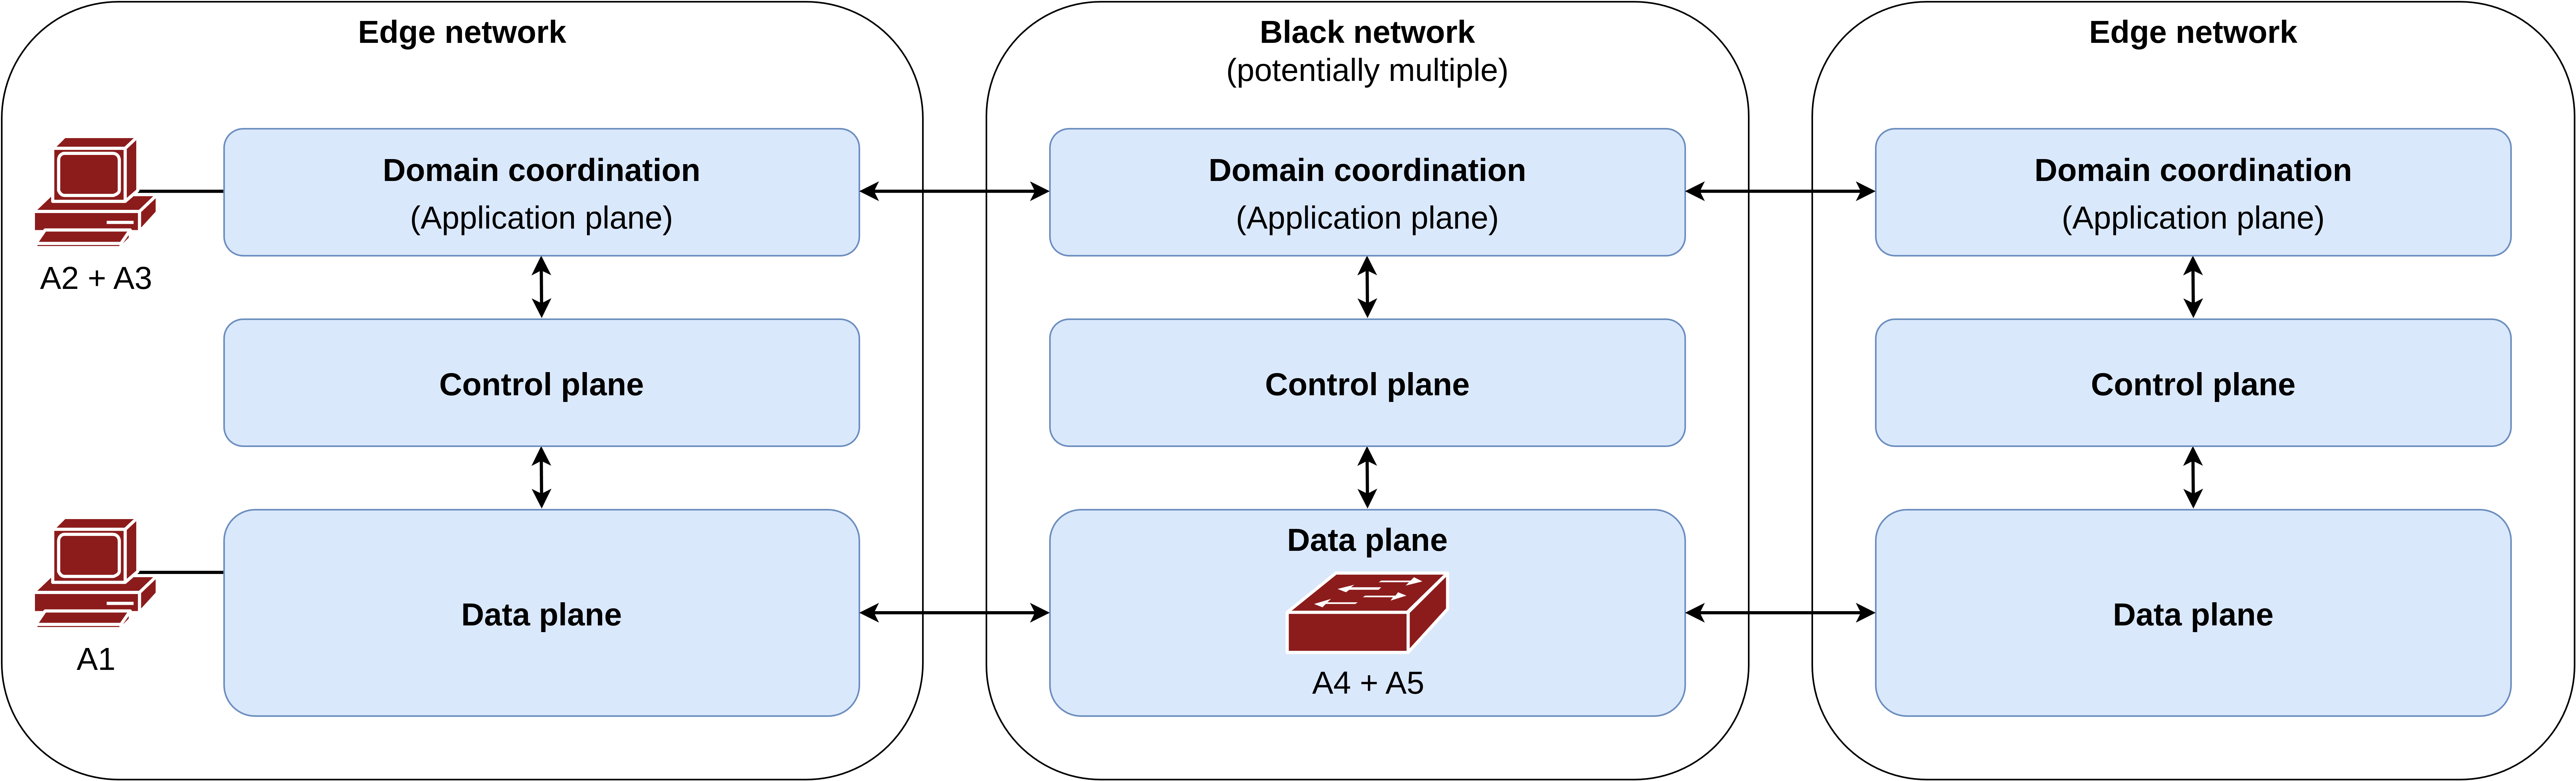
\includegraphics[width=\linewidth]{images/chapter_4/attacker_model.png}
        \caption[Attacker model]{Our attacker model indicating their location per domain and \acrshort{sdn} plane.}
        \label{fig:attacker_model}
    \end{figure}
%\end{landscape}